\chapter{Methodology and Data Gathering}
\label{chapter:methodology}
This thesis will be focused mainly on Classification problem of the "human presence" i.e. if the human is present or not. This will be a Supervised Learning problem where the features will be mapped to the classes/labels.
For this thesis, we are using VTT built 25 GHz RADAR.The methodology includes Data collection, Data cleaning, Model Building and Model deployment. Here is a flow, how the process will be conducted in the upcoming months.


\begin{figure}[ht]
  \begin{center}
    % below the size of the figure has been reduced for example
    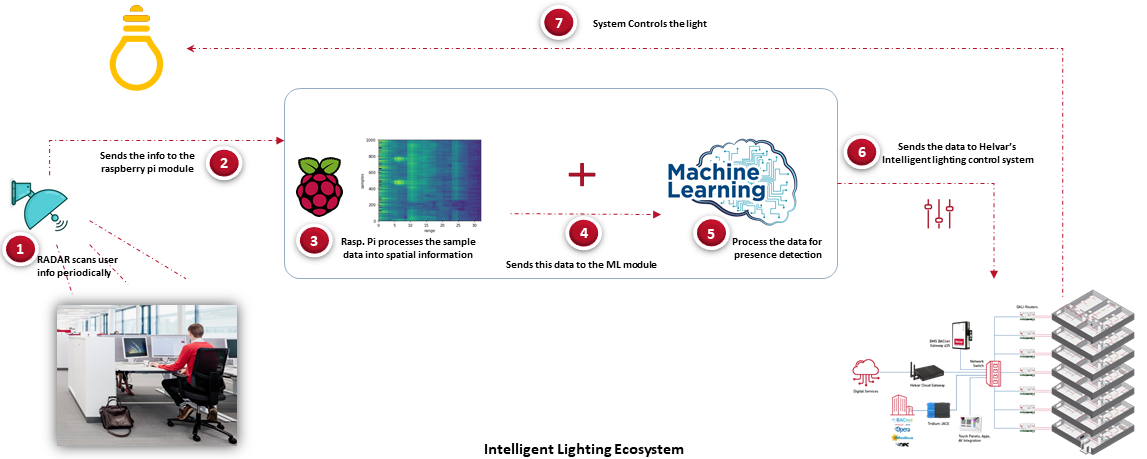
\includegraphics[width=1\textwidth]{Master's thesis/images/thesis_presentation.png} 
    \caption{Overall Process}
    \label{fig:basic_principle}
  \end{center}
\end{figure}


\begin{enumerate}
    \item RADAR box provides Analog to Digital converted signal. The data from these signals are collected over multiple hours at multiple locations.
    %However, this information is not sufficient to distinguish between human presence or absence. Therefore, in order to detect human presence i.e. to collect the labels for the data, we will be using RGB camera for the purpose of creating ground truth. RADAR data will be mapped with RGB presence detection based on each time frame.
    \item The data obtained will be feature engineered using multiple techniques.
    \item The idea is to engineer the received RADAR signal of every time frame (say 1 sec) to a 2-D map and then treating this 2-D map as an image or set of features.
    \item Deep Neural Networks or other Machine Learning techniques will be applied on this already processed data.
    \item For the purpose of training, we will leverage the cloud resources by AWS.
    \item The last step is to deploy these models on the edge devices.
\end{enumerate}

The ultimate objective is to create a more sustainable lighting control solution. Currently at Helvar, the most effective control system turns off the luminaires after 10 min of human absence. Even if, we are able to bring down these power wasteful windows by 50 \%, it would make huge impact on the society. Not only it will contribute to sustainability but will also result in lower power consumption and therefore less electricity bills. Lastly, it will add a lot of business value to Helvar as a company. In the following sections, we shall discuss the steps specified above in thorough detail.

\section{Experimental Design and Setup}

\subsection{Data Collection with RADAR}
RADAR itself cannot be used for direct communication with a workstation. That is why, Raspberry Pi 4 is used for communication. Raspberry Pi 4 acts as a mediator between the RADAR and a workstation through which data is being processed or analysed. 
The RADAR is connected to Raspberry Pi 4 internally and packed inside a 3D printed case, thus forming one module. Please be aware in further discussions, we will be referring this box i.e combination of RADAR and Raspberry Pi 4 as RADAR Box or just RADAR for the purpose of simplicity. When supplied power, the Raspberry Pi 4 inside the box opens a hot-spot for secure connection.The RADAR Box is then connected to the workstation using SSH. 

\begin{figure}[ht]
  \begin{center}
    % below the size of the figure has been reduced for example
    \includegraphics[width=0.5\textwidth]{Master's thesis/images/RADAR_int.jpg} 
    \caption{The RADAR Box - RADAR + Raspberry Pi4 }
    \label{fig:AoA}
  \end{center}
\end{figure}  

The program inside the Rpi to read data from RADAR is executed via this SSH. In order to send data from Rpi to the workstation, MQTT is used. The Message Queuing Telemetry Transport (MQTT) is a lightweight, publish-subscribe network protocol that transports messages between devices. It is designed for connections with remote locations where a ``small code footprint" is required or the network bandwidth is limited ~\cite{wikipedia_mqtt}. The hierarchy includes one broker and multiple clients. The broker receives all the messages from all the clients and then forwards to appropriate destinations. Information is organized in the form of topics. When a client publishes information on Topic A to broker, the broker sends this information to all the clients who have subscribed to this topic.

RADAR Box publishes information to a broker, and then broker sends the information to the workstation. The information received by the workstation is the actual received signals of the received antenna of the RADAR.  Instead of using a local workstation for storing the data, AWS S3 buckets are used for storing the data. AWS S3 is efficient method of storing as high volumes of data that can be easily accessed by people having the authorization.


%Data packet ( combination of chirps)
To dump the data to AWS, an efficient packaging technique for data was required. One Antenna of the RADAR generates 497 samples, i.e, 2x497 samples per chirp for two receiver antennas. In the basic raw mode, the time difference between two consecutive chirps is 31.25 ms. This means that the RADAR generates 2x497 samples in 31.25 ms or 32x2x497 samples in 1 sec. 
One way is to treat the signals of 1 chirp as one datum i.e one data sample with 2x497 feature vectors, however there is  a problem with this approach. For an instance time associated with this data is very less and features per chirp are not sufficient enough for our deep learning model to make an efficient prediction. Therefore, multiple chirps are stacked together to form one datum. In this thesis 32 chirps are stacked together to obtained one datum which represents 1 sec of signals. This approach will even make the labelling much easier which is explained in a more elaborate manner in the next section.

So in summary, the data produced every second is stacked together in the file format and then dumped to AWS S3 buckets. It is worth mentioning that the name of the file is the timestamp at which the first chirp was transmitted. This helps in storing the data properly and it makes it really simple to compare the data with an RGB camera, which will be explained in the next section.


\subsection{Ground Truth with RGB Camera}
\label{section:environments}
The RADAR is set to receive signals for the time span of 31.25 ms. This means in one second, an approximate of 32 signals are generated. The RADAR data is collected for multiple days in a meeting room of Helvar's headquarters in Espoo. This means on average, the RADAR generated 32x60x60x24 samples in 1 day. In an ever-moving environment like IT offices, its almost impossible to annotate such vast amount of data manually. It's not possible to label if a person was present or not for every second for the RADAR data manually.  One approach was to label the data using the meeting calendars i.e. label the data True if the meeting room is booked. But this approach is highly prone to false labelling. For an example, a meeting room can be occupied by a person even if its not booked. On the other hand, it may be possible that no one comes to the meeting the meeting room despite the booking. Therefore, the more reliable labelling mechanism was desired.

The other way to do was to record a video of the same at the same time of the RADAR and then using this video to annotate the data manually. This approach is again prone to a lot of loopholes, for e.g. manual annotation for days and days of data require a lot of extra effort. Apart from effort, this manual annotation method is really not scalable when we are dealing with commercial usage. It works fine for research based, but in an industry when eventually clients are involved, there is a need for exploring a better automatic solution. 

The data which is used in this thesis is hours and hours of data. In order to achieve reliable inference from our data, precise labelling is required for the training set. Therefore, for creating the labels for the RADAR data for training set, an RGB camera is used. Raspberry Pi 8.0 Mpix v2 camera with Sony IMX219 8-megapixel sensor is used for this thesis. The Camera Module can be used to take stills photographs as well as high-definition video. It supports 1080p30, 720p60 and VGA90 video modes, as well as still capture. The module is attached via a 15cm ribbon cable to the CSI port on the Raspberry Pi ~\cite{raspberrypi}.
\begin{figure}[ht]
  \begin{center}
    % below the size of the figure has been reduced for example
    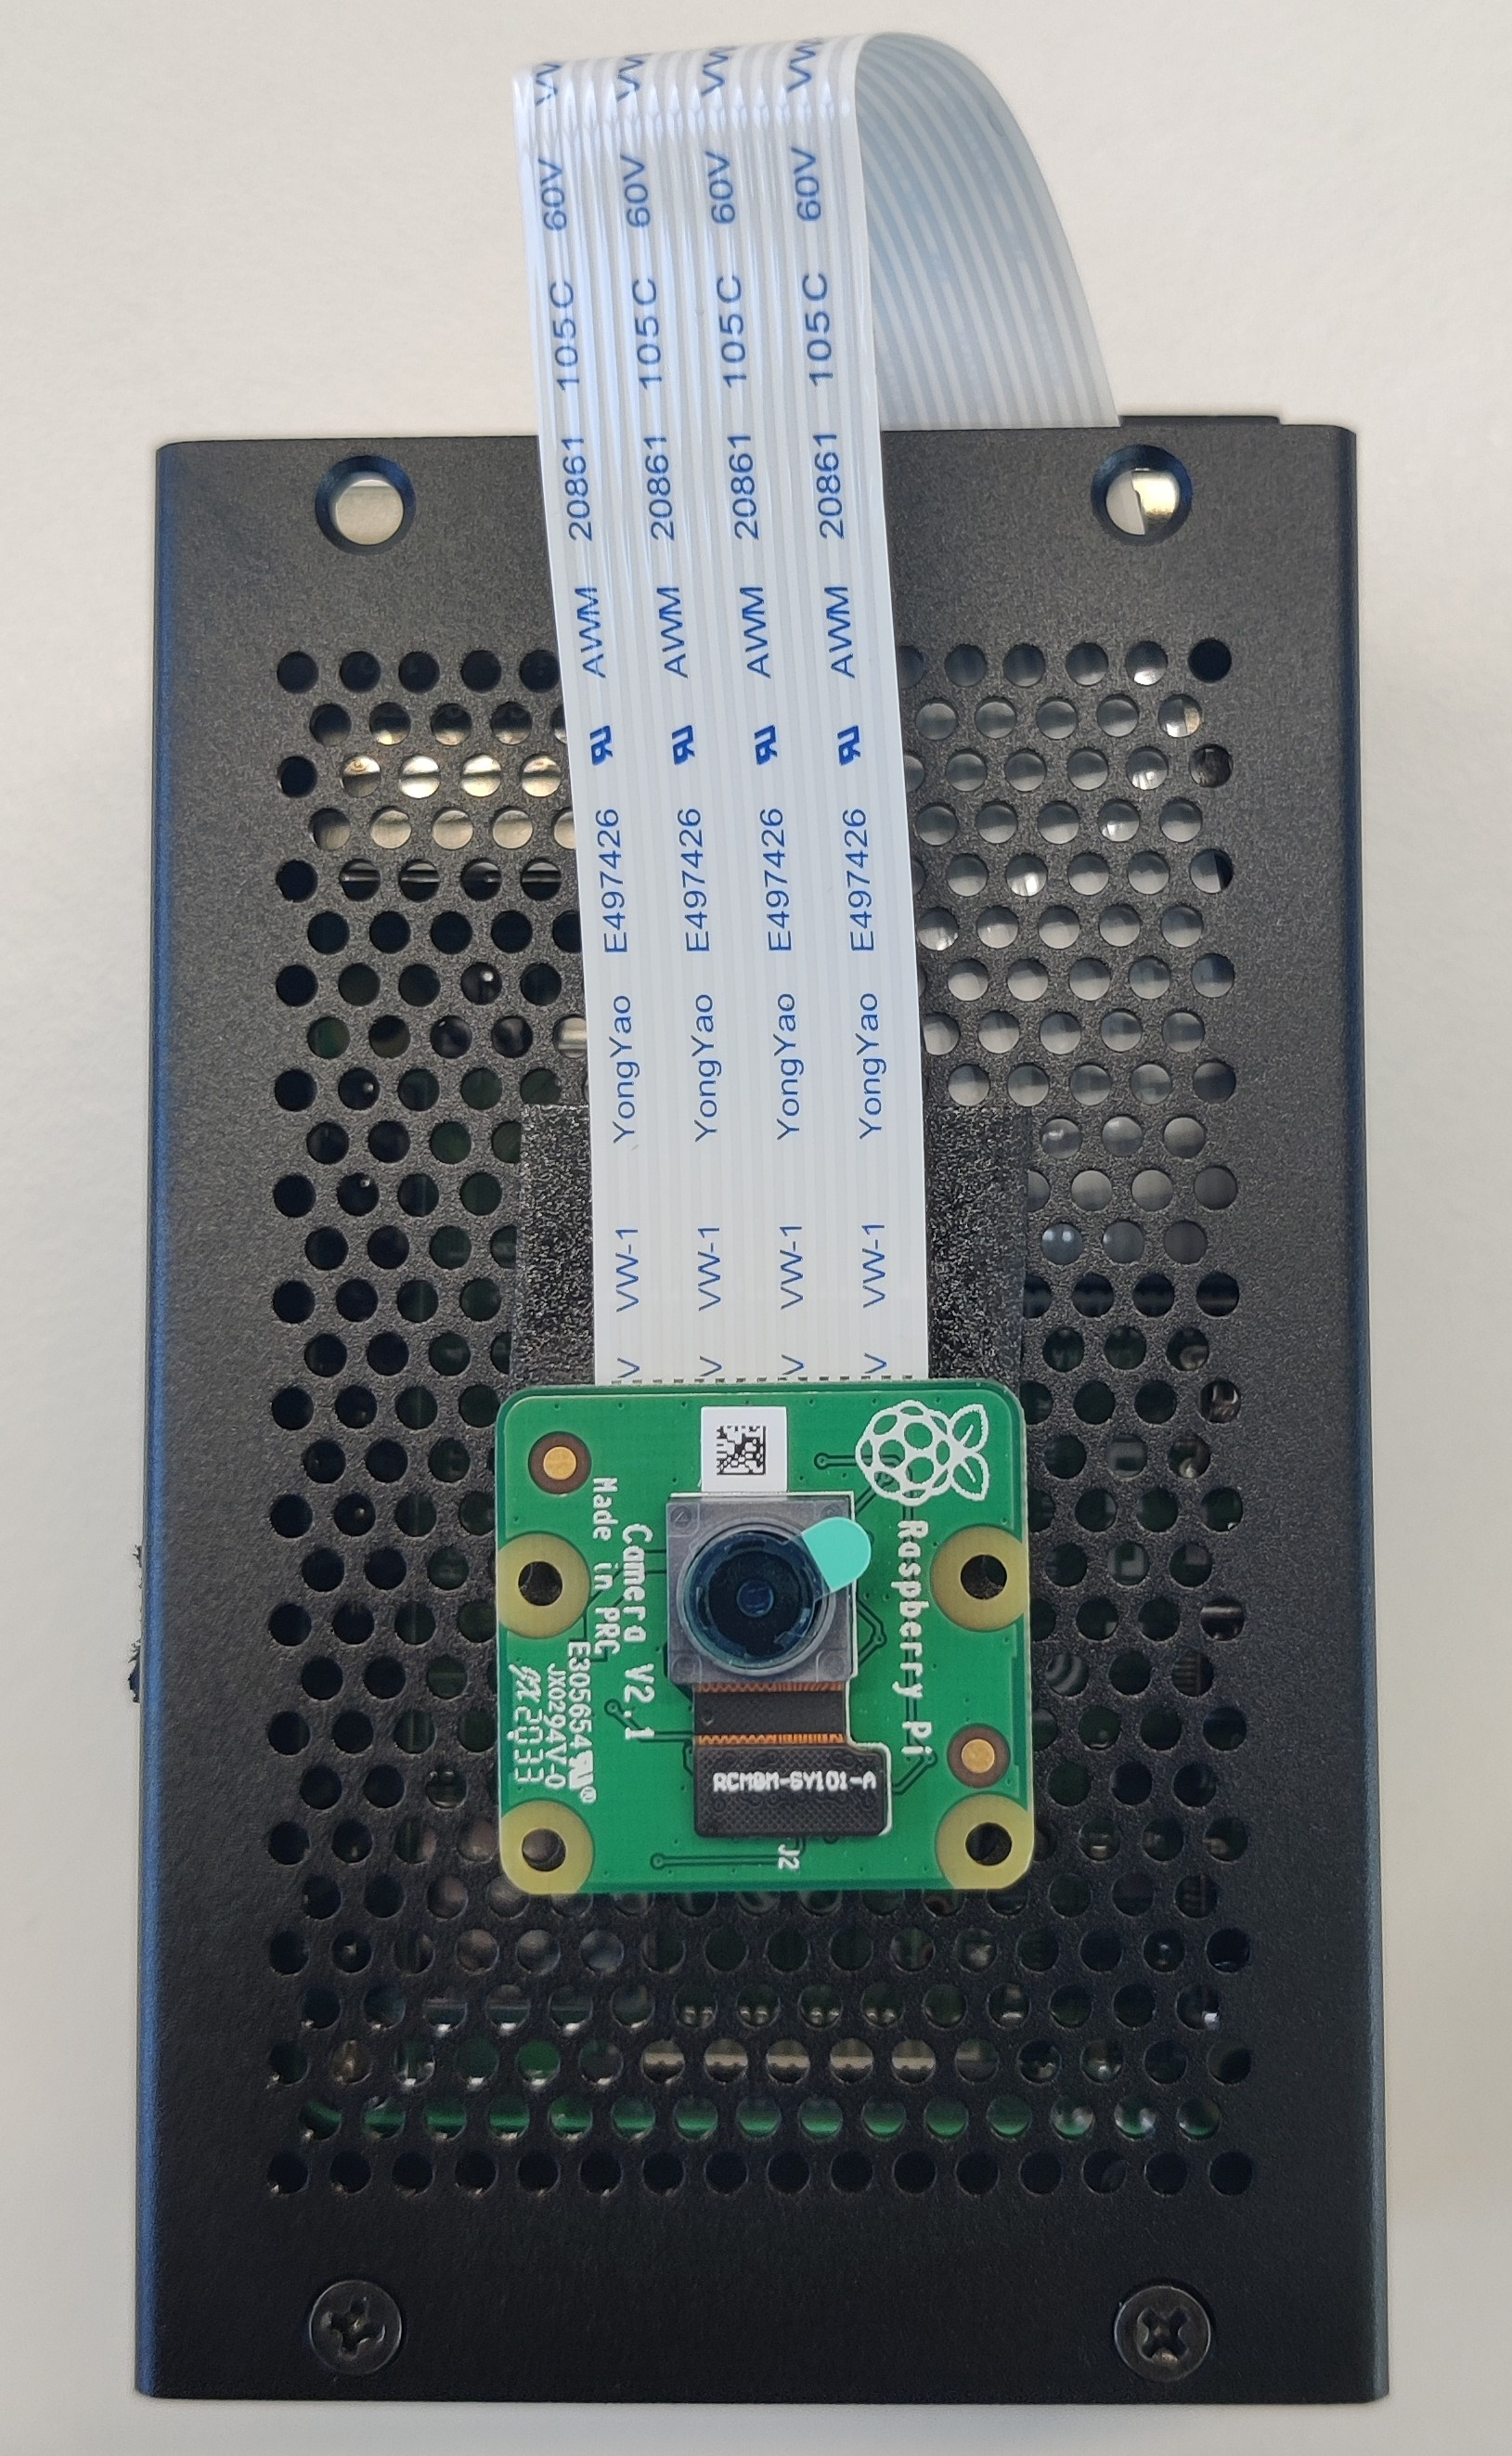
\includegraphics[scale = 0.07]{Master's thesis/images/RGB_camera.jpg} 
    \caption{The RGB Camera}
    \label{fig:AoA}
  \end{center}
\end{figure}  
However, instead of manually annotating these videos, the use cases of Machine Learning and Deep Learning are leveraged. With the advancement of Machine Learning and Deep Learning libraries, object detection and object recognition can be done with accuracy as high as 99\%. This field of Artificial Intelligence that trains computers to interpret and understand the visual world is called Computer Vision. With the advancement of AI and innovations in Deep Learning and Neural Networks, Computer Vision been able to take great leaps currently and has been able to surpass humans intelligence in some tasks related to detecting and labeling objects for optical sensors.


The RGB camera in the experiment and RADAR are mounted next to each other, so that the field of view of RADAR and camera overlaps. The camera used in this thesis captures 60 frames per second (fps). For the purpose of labelling the RADAR data, the scene is captured with an RGB camera alongside RADAR. The camera is connected to a 32-bit Raspberry pi 4. This Rpi leverages the camera to record videos. Each video file spans 1 second. The name of the file is the timestamp at which the file was created. As soon as the file is created, a parallel process dumps the data periodically to the AWS bucket. In order to prevent Rpi from memory overload, the files from the Rpi are removed as soon as they are dumped to AWS successfully. The important thing to notice here is the duration of the video. 1 sec is chosen so that it is easy later on to combine RADAR data as well RGB data. Once the data is dumped, the data is cleaned. For an instance, the videos of size 0 Kb are removed. These are the lost packets or the unsuccessful video captures.

\subsection{Platform for Collecting Data}
For this thesis, Data collected is huge. It is almost impossible for a local machine to run heavy computations on such a high volume of data. Therefore in order to run heavy computations without any memory leaks, the best possible technology available is the use of Cloud Resources. For the purpose of this thesis, we are using AWS EC2 instances. AWS EC2 instances are fast reliable and will be able to access the S3 buckets directly. 

There are different parameters to be taken into account while deciding to use CPU's or GPU's to train the deep learning models. Those parameters include the memory bandwidth, cost effectiveness and parallelism. GPU has on average better memory bandwidth in comparison to CPU's. Considering the data-set size, the larger the data-set the more advantage the GPU will have over CPU. As for the Parallelism of the model, some models have more parallelism than others. For example, Fast Forward Neural Networks (FNNs) and Convolutional Neural Networks (CNNs) can support high parallelism, therefore, it can be applied better on a Single Instruction Multiple Data (SIMD) processor such as the GPUs. Finally, coming to Cost-effectiveness, the power cost of GPU is higher than the CPU. For non parallel processes or less parallel processes like Recurrent Neural Networks, it is better to use a CPU. In this work, the cloud instances based on CPU or GPU is used to train the models according to the needs as mentioned above.

For this thesis, Deep Learning Base AMI Ubuntu instance of type p2.xlarge is used. Deep learning instance is launched in order to use the GPU instances for running the Deep Learning models. P2 instances provide up to 16 NVIDIA K80 GPUs, 64 vCPUs and 732 GiB of host memory, with a combined 192 GB of GPU memory, 40 thousand parallel processing cores, 70 teraflops of single precision floating point performance, and over 23 teraflops of double precision floating point performance ~\ref{amazonec2}. 


\subsection{Computing on Cloud for RGB Data}
\label{Computing on Cloud for RGB Data}

The data collected from RGB data which is stored in S3 buckets can be directly accessed from EC2 instance as both the instance and the bucket are present in the same AWS region.  For this project a hybrid of  two techniques are used for object detection on the RGB data collected. 
\begin{figure}[ht]
  \begin{center}
    % below the size of the figure has been reduced for example
    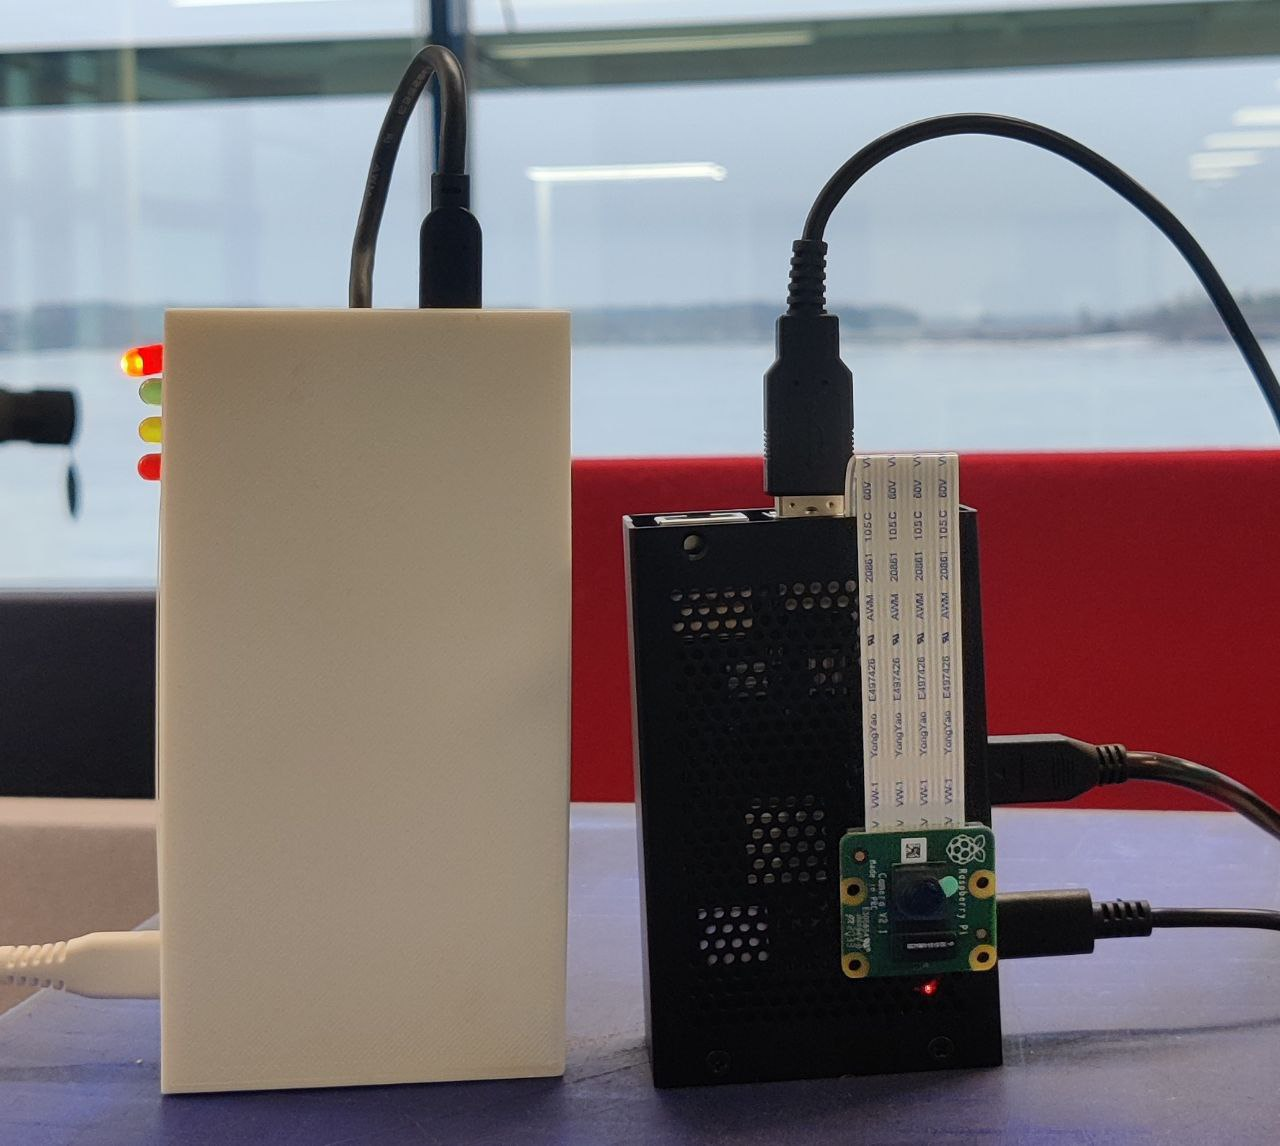
\includegraphics[width=0.5\textwidth]{Master's thesis/images/equipment.jpg} 
    \caption{RADAR and Camera}
    \label{fig:AoA}
  \end{center}
\end{figure}  
\begin{enumerate}
    \item \textbf{YOLOv3} - YOLOv3 is chosen because it is extremely fast and accurate. The mAP of YOLOv3 is measured at .5 IOU  which is on par with Focal Loss but about 4x faster. YOLOv3 uses a few tricks to improve training and increase performance, including multi-scale predictions, a better backbone classifier, and more ~\cite{yolo_time}. YOLOv3 returns output in the form of pre defined 80 classes on which the model is trained. Here in this thesis, only person class is a matter of interest. In order to detect only human, the detection class of the YOLOv3 model has been manipulated.
    \item \textbf{Motion Detection} - This technique is used to detect motion in a scene. It is used because sometimes it is possible for a person to be occluded in the video. For an instance, consider a person half occluded behind the desktop monitor, or a scenario where there is only hand moving in front of camera, or where someone is half visible behind the door, for such scenarios YOLOv3 will fail because there are a lot of occlusions present in the same. Therefore for such cases, motion detection algorithm is used on the RGB camera data. When the movement is beyond a fix threshold, only then the algorithm returns presence, otherwise it ignores small movements, for e.g.., movement due to curtains or leaves of the plants are ignored. The approach is very simple and self intuitive. When the program starts, it will capture a called baseline image. The program will keep comparing the new frame with this baseline image. If there is a movement in the new frame, the contents of the image will be different and if this difference is beyond a certain threshold,  the program will return Presence.
\end{enumerate}

Once the data is cleaned into AWS, YOLOv3 and  Motion Detector are run on the RGB data collected. Every second of collected data contains 60 frames, so for every second YOLOv3 and Motion Detector generates 60 labels. In the Lighting industry, the requirement for getting the true labels is within few seconds. The accuracy of milliseconds is not required in lighting industry. Therefore, for the sake of simplicity and better results, the mode value of the 60 labels was taken for every second. 

After using this pipeline, the labels corresponding to every second of RADAR data is ready. Its worth noticing that there might be some inaccuracies in the labelling because of the difference in the angle of view. 

\section{Transformations and Data visualization of RADAR Data}

In the previous section, we talked about how the pipelines are arranged for the proper flow of data. In this section, we will talk about how the data is arranged for the machine learning model to work efficiently. This section will also explain the operations and transformations done on the data. In addition to that, we will see exploratory data analysis done on the radar data.

The data from FMCW RADAR is generated in the form of chirps/sweeps. According to the hardware configuration of the RADAR used in this thesis, it generated 497 samples in one chirp. Since the RADAR have two receiver antennas, it generates 497 per antenna in 1 chirp. RADAR generates 1 chirp is approximately 31.25 ms, although the time may vary in fractions of milliseconds. This means the RADAR generates approximately 32 samples in 1 second. On the other hand, the RGB camera operates at 60 fps. In order to overlap the data and make an effective labelling, the data from 32 chirps of RADAR is combined together to make a combined signal of 1 second. Alternately, it can be imagined that one instance of data for our Machine Learning/Deep Learning model corresponds to 1 sec of data, i.e. 32 sweeps from the RADAR and 60 frames of camera are mapped together. Therefore the data signature of the RADAR of 1 second can be imagined as a 3D matrix where first dimension corresponds to antenna number, second dimension corresponds to chirp number and the third dimension corresponds to Time. The value of cell is the actual amplitude of the signal. Timestamping is used for mapping of RADAR and RGB camera data. These 1 second videos of RGB camera when fed to YOLOv3 and Motion detector model, as explained in the previous subsection \ref{Computing on Cloud for RGB Data}, generates output in the form of True/False. 
\begin{figure}[ht]
  \begin{center}
    % below the size of the figure has been reduced for example
    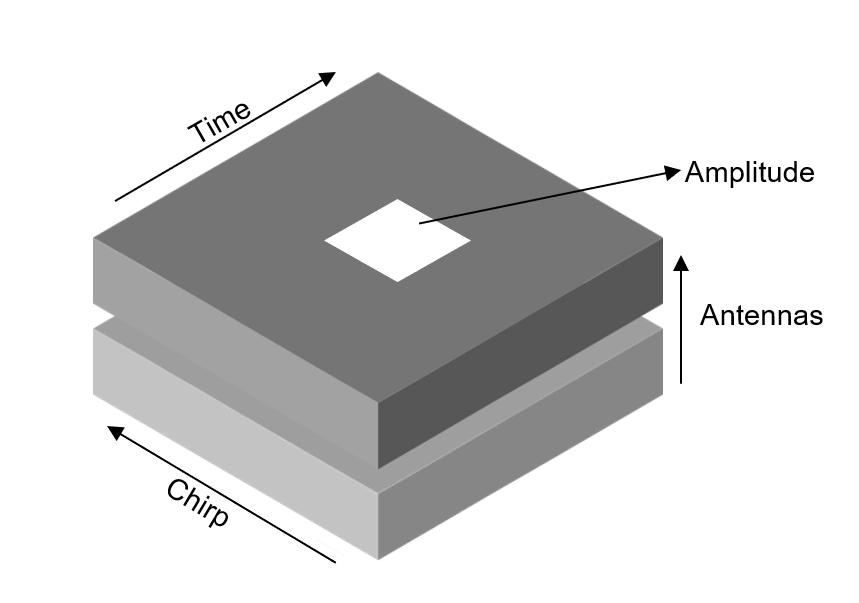
\includegraphics[width=0.5\textwidth]{Master's thesis/images/signature.PNG} 
    \caption{The data signature for RADAR}
    \label{fig:signature}
  \end{center}
\end{figure}  



In the Fig. \ref{fig:raw_signal}, random instances of RADAR data are sampled. Every plot corresponds to 1 second of data. The data from 32 chirps is flattened to make it a Time vs Amplitude plot. Since each chirp has 497 samples, therefore the Time axis has $32\times497$ samples on the x axis. The y axis corresponds to Amplitude of the received signal. The title of the subplots presents if there was presence or absence in the RADAR view. False corresponds to absence while Presence corresponds to Presence. Clearly there is significant difference between presence and absence. The signals from absence scenario is similar across time, or we can say that time does not change the signal. However it is completely different in presence scenario, the signal tend to change a lot over time.

\begin{figure}[ht]
  \begin{center}
    % below the size of the figure has been reduced for example
    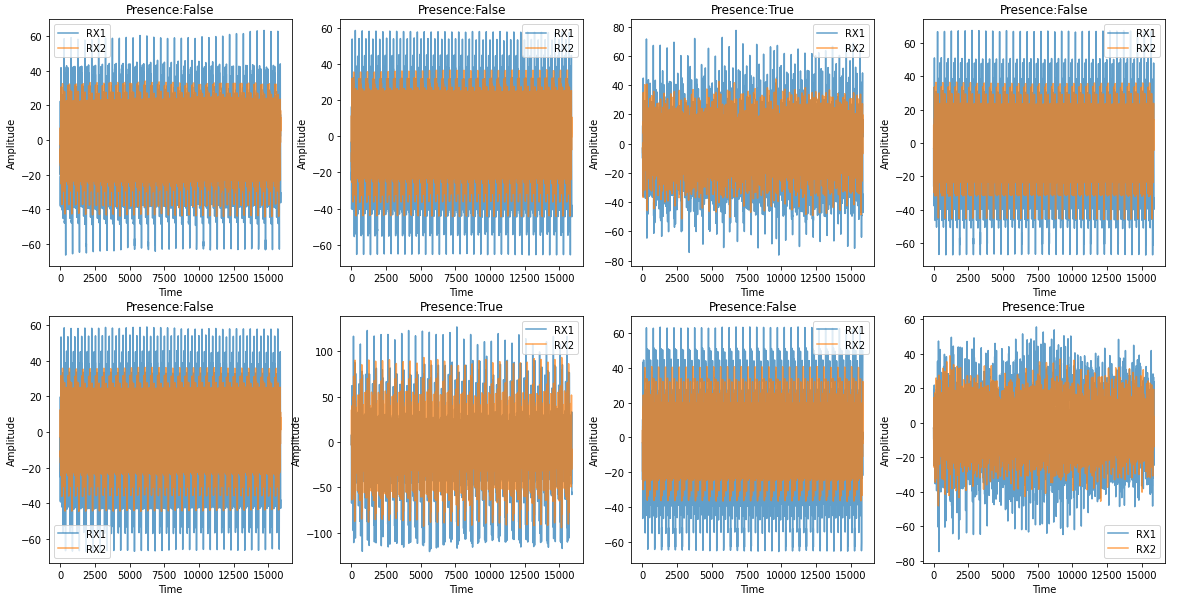
\includegraphics[width=01\textwidth]{Master's thesis/images/raw_signal.PNG} 
    \caption{Random sampling of 1 second of RADAR data}
    \label{fig:raw_signal}
  \end{center}
\end{figure}  

Deep learning models were tried directly using this raw data. However the model prediction was not highly accurate. One reason could be significant difference in amplitude in different scenarios. The amplitude differs a lot based on the range, and range of objects varies from scenario to scenario. Therefore the raw data can not be used directly for ML models. The second reason for not using this raw data directly for ML model is the maximum range capacity. The RADAR data in its raw form can detect objects up to 250 metres. But in an office environment, we really do not need data beyond some threshold. The data beyond this threshold will be just noise. The third reason is, the data in raw form has a lot of noise due to cluttering. The SNR for raw data is heavily compromised in raw form. Therefore, some transformations were required on this data for the ML model to work properly.

As explained in subsection \ref{Signal Processing for FMCW}, the data was converted from $Time\times Amplitude$ to $Range\times Amplitude$ using Fourier Transformation. As explained earlier, Fourier Transformation converts the Time into Frequency. Since in FMCW RADAR frequency directly estimates the Range, that is why Time gets converted to Range. This transformation is called \textbf{Range FFT}. Here FFT means Fast Fourier Transformation, which is a faster method of computing Fourier Transformations of discrete signal.

A very common problem associated with FFT is \textbf{Spectral Leakage}. An estimation of a signal computed using FFT or DFT does not contain spikes and zeros like shown in Fig. \ref{fig:comp_fft}, instead it will have a dominant peak which is then smudged over several consecutive bins. It happens because of finite window of data as the data is never infinitely large. In order to cater to this problem, windowing functions are used to reduce the spectral leakage. In this thesis \textbf{Blackman Window} is used. It is designed to have close to the minimum leakage possible. The Blackman window is defined as,
\begin{equation*}
    w(n) = 0.42 - 0.5\cos(2\pi n/M) + 0.08\cos(4\pi n/M)
\end{equation*}
where \(M\) is the number of samples and \(n\) is the $n^{th}$ sample. It is also known as an apodization which means ``removing the foot", i.e. smoothing discontinuities at the beginning and end of the sampled signal or tapering function \cite{blackman1958measurement}\cite{oppenheim2010discrete}.

Once the Blackman windowing is applied to raw data, FFT of the data is computed. The result of the FFT is then normalized to make the Euclidean norm of the signal equal to 1. Range FFT returns 512 samples( closest to 497), out of which half the samples are mirror images. But for the sake of putting an upper limit on the range i.e. to what range we want to detect objects, we have put an upper limit of 32 samples. This number 32 has been chosen after considerable number of experiments. These 32 samples corresponds roughly to 18.7 metres. 
\begin{figure}[ht]
  \begin{center}
    % below the size of the figure has been reduced for example
    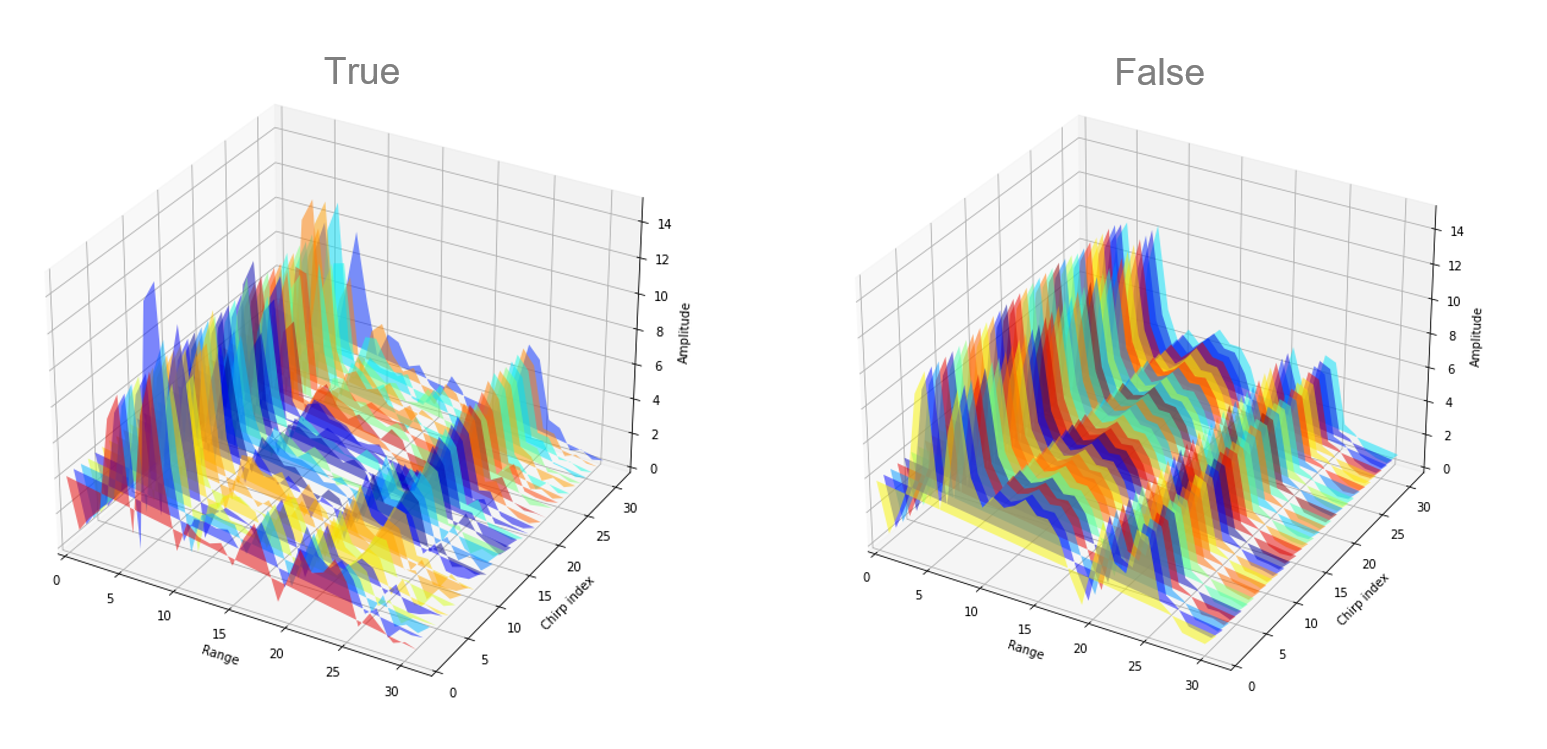
\includegraphics[width=1\textwidth]{Master's thesis/images/fft_p_a.PNG} 
    \caption{Range FFT comparison for human presence and absence with one receiver antenna}
    \label{fig:FFT_3d1a}
  \end{center}
\end{figure} 
Fig. \ref{fig:FFT_3d1a} represents a 3 dimensional view of Range FFT data. A comparison of the Range FFT signal for human presence and absence is done in the figure. It is worth mentioning that the plot indicates the Range FFT output of only one antenna. Similar signal is obtained from the another antenna as well. 
It is very evident from the plots that in the scenario when there was no human, the signal remain constant over chirps. However when there was human movement involved, the signal varies over chips. Every plot corresponds to 1 second of data. It i worth noticing that the y axis which corresponds to chirp index ranges from 0 to 32, and the Range axis also ranges from 0 to 32 on the x axis.

\begin{figure}[ht]
  \begin{center}
    % below the size of the figure has been reduced for example
    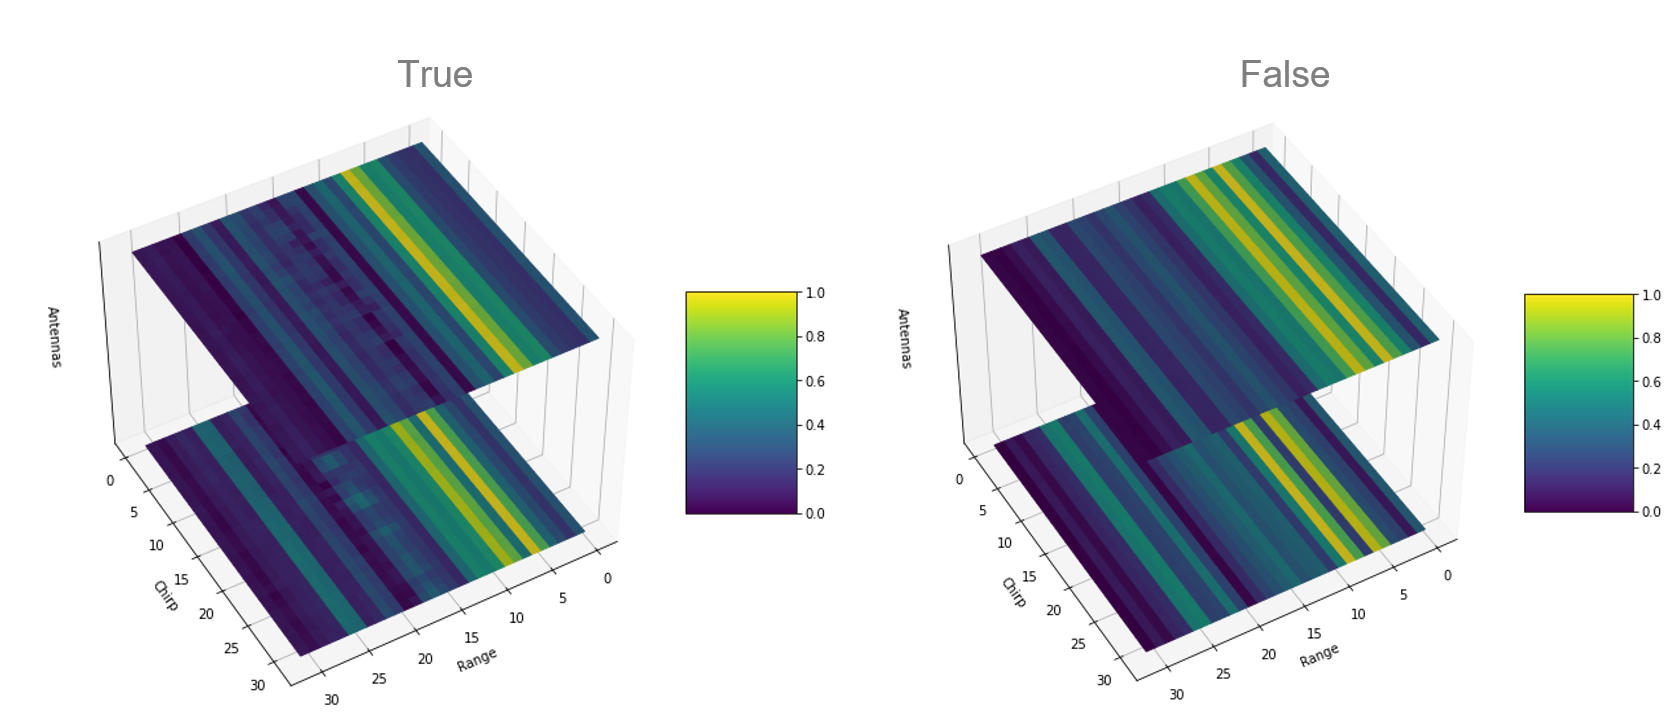
\includegraphics[width=1\textwidth]{Master's thesis/images/4d_fft.PNG} 
    \caption{Range FFT comparison for human presence and absence with both receiver antenna}
    \label{fig:FFT_4d2a}
  \end{center}
\end{figure}   

To visualize this scenario even better, a 4 dimensional plot is drawn involving 2 antennas in Fig. \ref{fig:FFT_4d2a}. The color in the plots indicates the amplitude intensity. Yellow color corresponds to higher amplitude values and blue corresponds to lower amplitude values. It is evident in the plots that the amplitude values of the two antennas are always comparable in quantification. It can be seen in this plot as well that in the scenario of human absence, the amplitude of the signal remains constant across chirps. Comparatively in the human presence scenario, a distinctive smudge can be observed across chirps. This also comes by intuition that when the human movement in involved, a human body, which is a collection of points, is at different distance from the RADAR. It is important to note that the distance from one antenna is of course different than the distance from another antenna, but the difference is diminutive as the antennas are placed in close proximity.
\begin{figure}[ht]
  \begin{center}
    % below the size of the figure has been reduced for example
    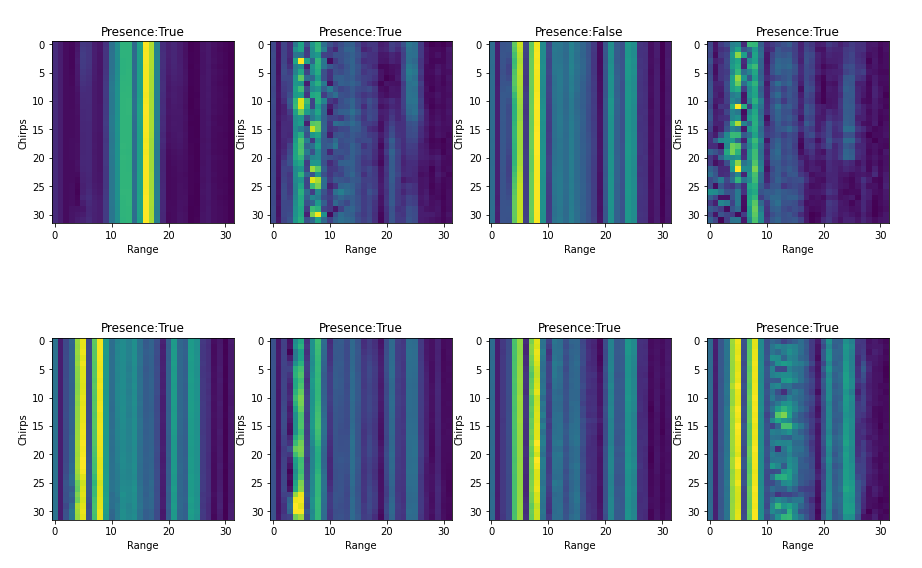
\includegraphics[width=01\textwidth]{Master's thesis/images/fft_1_antenna.PNG} 
    \caption{Range FFT on random randomly sampled RADAR data}
    \label{fig:FFT_plot}
  \end{center}
\end{figure}  
\begin{figure}[ht]
  \begin{center}
    % below the size of the figure has been reduced for example
    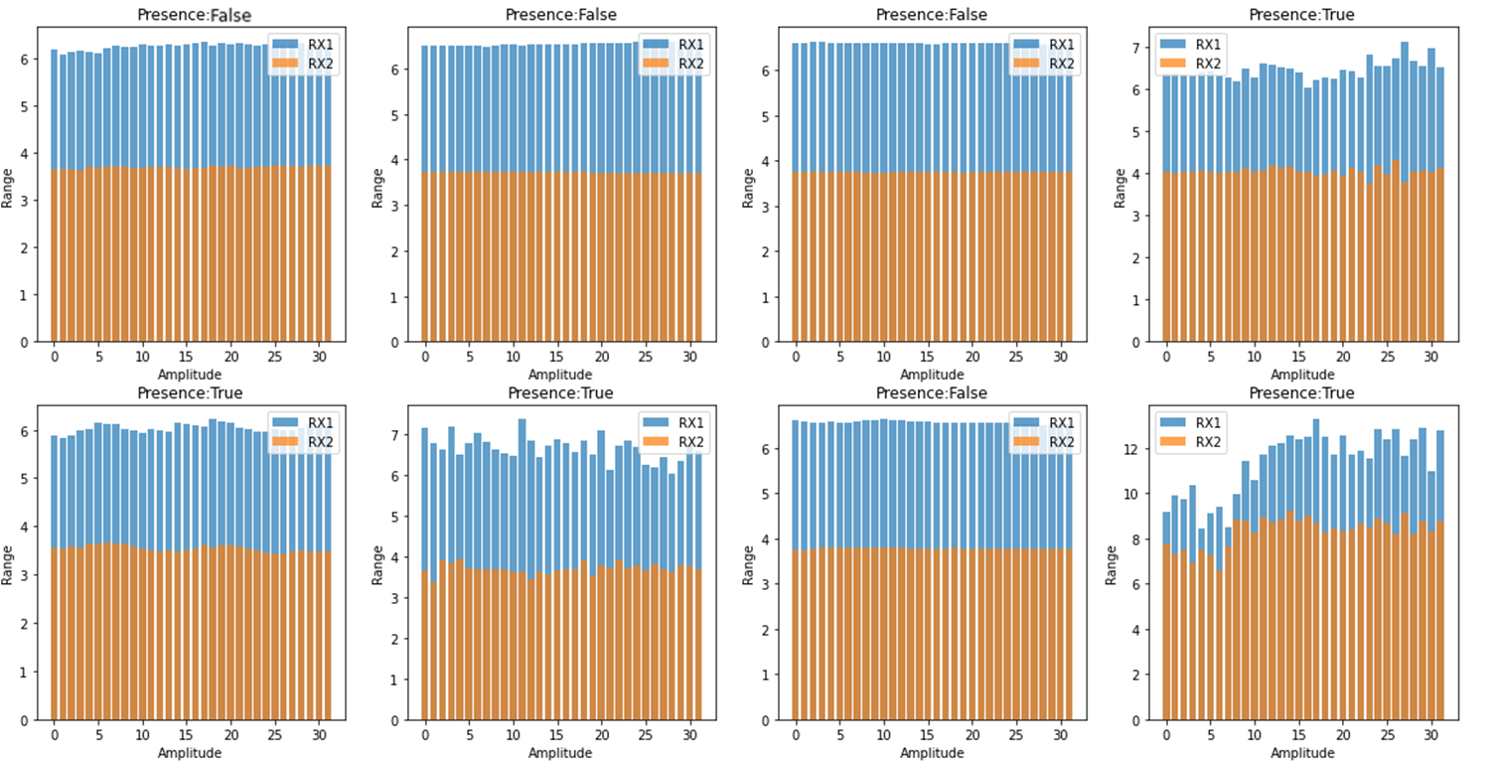
\includegraphics[width=01\textwidth]{Master's thesis/images/ff_bar.png} 
    \caption{Amplitude vs Range Bar Chart for both the antennas where Amplitude is the mean value within 1 chirp}
    \label{fig:FFT_bar}
  \end{center}
\end{figure}
In Fig. \ref{fig:FFT_plot}, random instances of the Range FFT are sampled to display how data from Range FFT looks like. The subplots indicates presence and absence scenario. The plot indicates results from only one antenna as the interpretation is much easier for one antenna. The other antenna gets the same results. The important thing to notice here is that, these plots are obtained from different locations, i.e, from meeting rooms, from open office and from desk premise. This fact is evident from the plot itself. For e.g. highest intensity does not remain in the same range. For some scenarios the highest intensity bins are generated by objects closer to the RADAR, while in some scenarios, the highest intensity bins are generated by objects far from RADAR. Additionally we can observe the smudge in the Range FFT which we discussed above can be seen clearly. The smudge can be seen in all the human presence scenarios irrespective of where the data was collected. 

To analyze it even further, the bar plot is drawn by taking the average value per chirp which can be seen in Fig. \ref{fig:FFT_bar}. Every chirp will give one mean amplitude value, giving rise to 32 mean amplitude values corresponding to 32 chirps. This is done for both the RX antennas. The objective behind this plot is to analyze if the mean value stays constant over chirps in absence scenario and vary over chirps in present scenario. Result can be interpreted clearly in the absence scenario (indicated by False), where the mean amplitude value remains constant for both the antennas. This result is very intuitive as there is no movement, so all the chirps gets the same signal.

Deep learning models were tried on Range FFT data. However the model prediction was not highly accurate. One reason could be significant difference in amplitude in different scenarios. The amplitude differs a lot based on the range, and range of objects varies from scenario to scenario. Therefore the Range FFT can not be used directly for ML models. Another reason is the scenario when there is little movement across chirp. The gradient is so less that the Machine Learning model assumes small movement as a background noise. There more transformation is required to capture these small movements and thus increasing SNR.

As explained in subsection \ref{Signal Processing for FMCW}, the Range FFT was further converted from $Range\times Amplitude$ to $Range\times Velocity$ using another Fourier Transformation. This transformation is called \textbf{Range-Doppler FFT} since Doppler FFT is applied on Range FFT. As explained earlier, Fourier Transformation converts the Chirp index into Velocity. \textbf{The advantage of using Doppler FFT is that}. It is worth noting that in case of absence scenario, all the values in the Range Velocity matrix will be zero or near to zero as there is no movement in the scene.
\begin{figure}[ht]
  \begin{center}
    % below the size of the figure has been reduced for example
    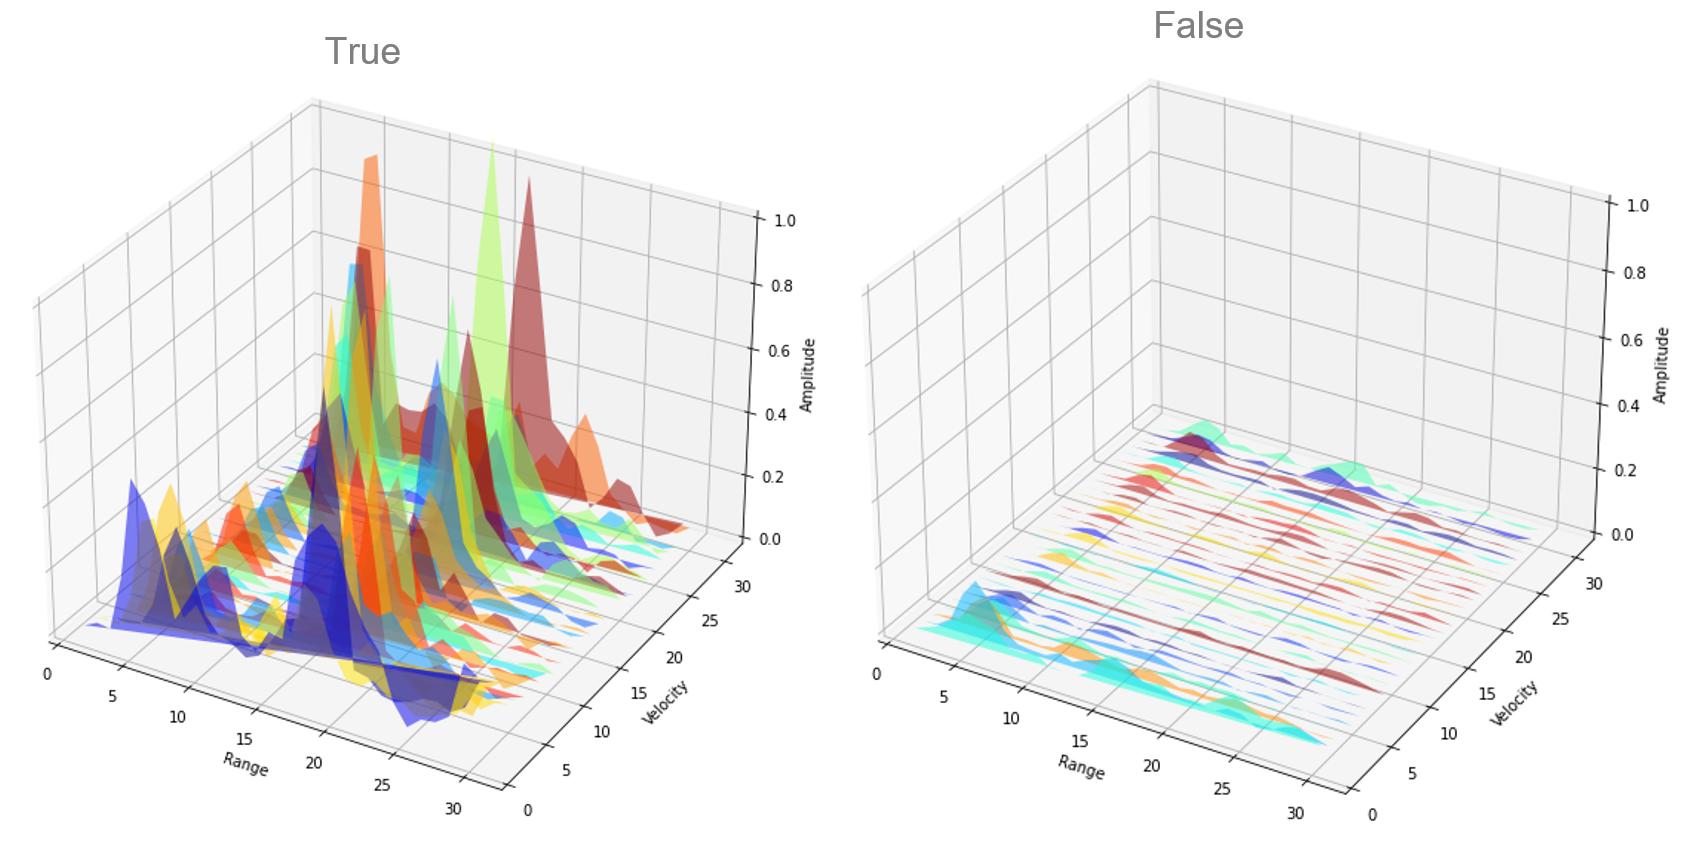
\includegraphics[width=1\textwidth]{Master's thesis/images/2ndFFT.PNG} 
    \caption{Range FFT comparison for human presence and absence with one receiver antenna}
    \label{fig:rdFFT_3d1a}
  \end{center}
\end{figure} 
Fig. \ref{fig:FFT_3d1a} represents a 3 dimensional view of Range FFT data. A comparison of the Range FFT signal for human presence and absence is done in the figure. It is worth mentioning that the plot indicates the Range FFT output of only one antenna. Similar signal is obtained from the another antenna as well. 
It is very evident from the plots that in the scenario when there was no human, the signal remain constant over chirps. However when there was human movement involved, the signal varies over chips. Every plot corresponds to 1 second of data. It i worth noticing that the y axis which corresponds to chirp index ranges from 0 to 32, and the Range axis also ranges from 0 to 32 on the x axis.

\begin{figure}[ht]
  \begin{center}
    % below the size of the figure has been reduced for example
    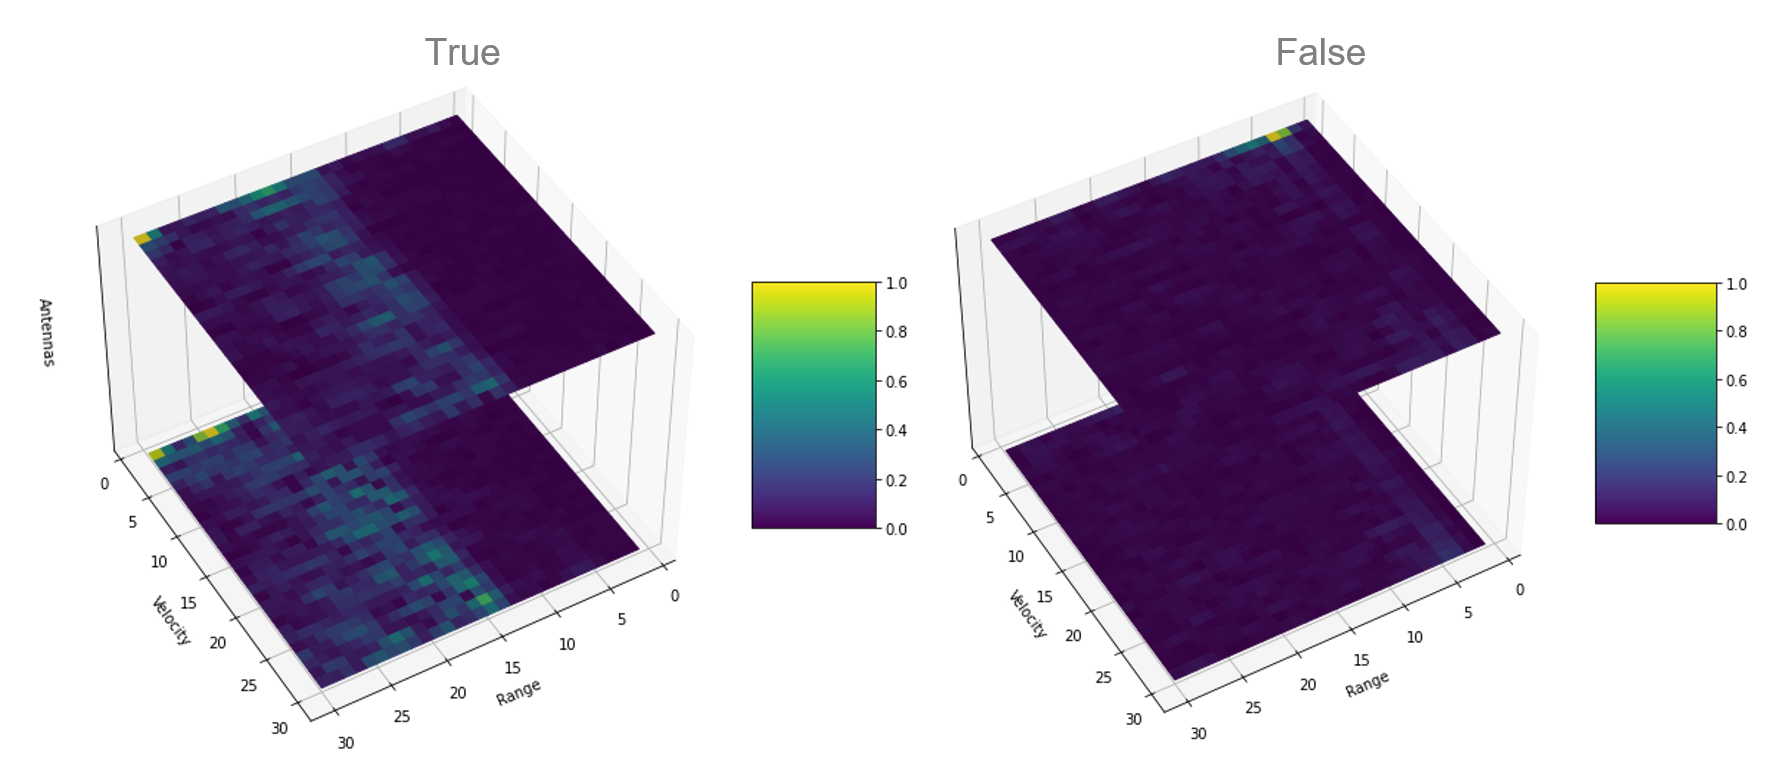
\includegraphics[width=1\textwidth]{Master's thesis/images/4d_rdfft.PNG} 
    \caption{Range FFT comparison for human presence and absence with one receiver antenna}
    \label{fig:rdFFT_4d2a}
  \end{center}
\end{figure} 